\documentclass[a4paper,12pt]{article}

\usepackage{graphicx}   % Imágenes
\usepackage{helvet}     % Fuente de letra
\usepackage[hidelinks]{hyperref}   % Tabla de contenido
\usepackage{url}
\usepackage{etoolbox}
\usepackage{setspace}   % Interlineado
\usepackage{geometry}   % Márgenes
\usepackage{tabularx}   % Tablas

% Márgenes
\geometry{
    a4paper,
    left=25mm,
    right=25mm,
    top=25mm,
    bottom=25mm
}

% Eliminar título de la bibliografía
\patchcmd{\thebibliography}{\section*{\refname}}{}{}{}

\onehalfspacing

\renewcommand{\familydefault}{\sfdefault}
\renewcommand{\contentsname}{Tabla de contenidos}

% Configuración de la portada
\begin{document}

\begin{titlepage}
    \centering
    \vspace*{0.5cm}

    % Logo de la universidad
    
\includegraphics[width=1\textwidth]{logo-tec.png}\par\vspace{1cm}

    % Nombre de la universidad
    {\scshape Instituto Tecnológico de Costa Rica\par}
    \vspace{2cm}

    % Título
    {\Huge\bfseries Proyecto \#1: Scanner\par}
    \vspace{2cm}

    % Escuela
    {\large Escuela de Ingeniería en Computación\par}

    % Curso
    {\large Compiladores e Intérpretes IC-5701\par}
    \vspace{2cm}

    % Autor
    {\large Alonso Navarro Carrillo, c. 2022236435\par}
    \vspace{0.25cm}
    {\large Carlos Venegas Masis, c. 2022153870 \par}
    \vspace{0.25cm}
    {\large Valeria, c. \par}
    \vspace{2cm}

    \vfill

    % Profesor
    {\large Ing. Ericka Marín Schumann\par}

    % Semestre
    {II Semestre 2024\par}
\end{titlepage}

\tableofcontents\newpage

% Introducción
\section*{Introducción}
\addcontentsline{toc}{section}{Introducción}
\begin{flushleft}
	\hspace*{2em} Este proyecto se sitúa en la primera etapa del desarrollo
de un compilador para el lenguaje de programación C, conocida como el
Análisis Léxico. El objetivo principal de esta etapa es diseñar y construir
un scanner que sea capaz de identificar y clasificar los diferentes tokens
que conforman un programa en C. Para lograr esto, se utilizó la herramienta
JFlex, la cual permite definir expresiones regulares que describen los patrones
de los tokens a reconocer.\par
\vspace{1em}
\hspace*{2em} A lo largo de este documento se detalla el proceso de desarrollo 
del scanner, desde la planificación hasta la implementación y evaluación de los
resultados obtenidos. Se describen decisiones técnicas tomadas para garantizar el
correcto funcionamiento del proyecto, así como las estrategias empleadas para la 
solución de los problemas encontrados durante su desarrollo. 

\end{flushleft}

% Estrategia de solución
\section*{Estrategia de solución}
\addcontentsline{toc}{section}{Estrategia de solución}
\begin{flushleft}
    \hspace*{2em} Después de leer detenidamente la documentación 
    de JFlex, se comenzó a diseñar las expresiones regulares 
    para los tokens que debía reconocer el escáner. Aquí surgió 
    el primer problema: el escáner reconoce los tokens según 
    el orden de prioridad. Es decir, si la primera expresión 
    regular es un punto, ningún otro token será reconocido, 
    ya que este metacaracter coincide con cualquier carácter, 
    interpretándolo como un error. Por lo tanto, fue crucial 
    definir adecuadamente el orden de las expresiones regulares. \par
    \vspace{1em}
    \hspace*{2em} Una vez definido el orden de las expresiones 
    regulares, procedimos a diseñar la estructura de los tokens 
    y sus tipos. Para ello, decidimos crear un mapa que facilitara 
    la búsqueda de tokens repetidos en el documento. De manera 
    similar, cada token guarda las líneas en las que aparece 
    en un mapa, lo que permite incrementar el contador de 
    ocurrencias de un token en una misma línea. Finalmente, 
    los tipos de tokens se almacenan en un enum. \par
    \vspace{1em}
    \hspace*{2em} Por último, se implementaron errores 
    definidos, como un número seguido de un identificador 
    o números flotantes que comienzan con un punto. Era 
    necesario definir estos errores como tokens para que 
    pudieran ser reconocidos por el escáner. Los errores no 
    se almacenan en una estructura de datos; en su lugar, se 
    imprimen directamente y no se agregan al mapa de tokens. \par
    \vspace{1em}
\end{flushleft}

\newpage

% Análisis de resultados
\section*{Análisis de resultados}
\addcontentsline{toc}{section}{Análisis de resultados}
\begin{table}[!ht]
    \centering
    \begin{tabularx}{\textwidth}{|X|X|X|}
        \hline
        Actividad & Porcentaje realizado & Justificación \\ 
        \hline
        Desplegar lista de errores léxicos & 100\% & \\
        \hline
        Desplegar listado de tokens encontrados & 100\% & \\
        \hline
        Mostrar tipo de token, línea y cantidad de apariciones por cada token & 100\% & \\
        \hline
        Manejar 4 tipos grandes (operadores, literales, ids, palabras reservadas) de tokens & 100\% & \\
        \hline
        Ignorar comentarios en línea y bloque & 100\% & \\
        \hline
        Identificar todos los operadores válidos de C & 100\% & \\
        \hline
        Identificar todos los literales válidos de C & 100\% & \\
        \hline
        Identificar todos los identificadores válidos de C & 100\% & \\
        \hline
        Identificar todas las palabras reservadas de C & 100\% & \\
        \hline
        Definir errores léxicos & 100\% & \\
        \hline
    \end{tabularx}
\end{table}

% Lecciones aprendidas
\section*{Lecciones aprendidas}
\addcontentsline{toc}{section}{Lecciones aprendidas}

% Casos de prueba
\section*{Casos de prueba}
\addcontentsline{toc}{section}{Casos de prueba}
\subsection*{Caso de prueba 1: Comentarios}
\addcontentsline{toc}{subsection}{Casos de prueba 1: Comentarios}
\begin{flushleft}
    \begin{verbatim}
    #include <stdio.h> // Comentario después de directiva de preprocesador
    #define MAX(a, b) ((a) > (b) ? (a) : (b)) // Macro con comentario en línea 
        
    // Este es un comentario en línea
    int main() {
        // Comentario con caracteres especiales: !@#$%^&*()
        /* Comentario en bloque con caracteres especiales: !@#$%^&*() */
        // Comentario con código incorrecto: int x = ;
        /* Comentario en bloque con código incorrecto: int y = ; */
        // Comentario con    espacios
        /*  Comentario en     bloque con espacios */
        //      Comentario con tabulaciones
        int a = 10; // Comentario al final de una línea de código
        int b = 20; /* Comentario en bloque
                        que se extiende en varias líneas */ 
        int d = a + b;
        int c = a + b; // Comentario después de una expresión 
        char *str = "Este es un string con // comentario en línea";
        char *str2 = "Este es otro string con /* comentario en bloque */";
        b = 20;
        /* Comentario en bloque sin cerrar
        b = 20; // Comentario en línea anidado
        return 0;
    }
    \end{verbatim}
    Errores esperados:
    \begin{itemize}
        \item Error en la línea 1: Operador inválido '\#'.
        \item Error en la línea 2: Operador inválido '\#'.
        \item Error en cáscada en línea 20: Comentario de bloque sin cerrar.
    \end{itemize}
    \hspace*{2em} Es importante resaltar que aunque el proyecto indique que no se pueden 
    tener errores en cáscada, al encontrar un comentario de bloque sin cerrar el comportamiento
    usual será seguir buscando hasta encontrar un "*/".\par\vspace{1em}
    Resultados:
    \begin{verbatim}
Errors: 
Character unknown: # in 1
Character unknown: # in 2
Block comment without closure: /* Comentario en bloque sin cerrar
    b = 20; // Comentario en linea anidado
    return 0;
} in 20
+------------+-----------------+------------------------------------------+
| Token      | Tipo de Token   | Linea                                    |
+------------+-----------------+------------------------------------------+
| char       | KEYWORD         | 17, 18                                   |
+------------+-----------------+------------------------------------------+
| int        | KEYWORD         | 5, 13, 14, 15, 16                        |
+------------+-----------------+------------------------------------------+
| MAX        | ID              | 2                                        |
+------------+-----------------+------------------------------------------+
| a          | ID              | 2(3), 13, 15, 16                         |
+------------+-----------------+------------------------------------------+
| b          | ID              | 2(3), 14, 15, 16, 19                     |
+------------+-----------------+------------------------------------------+
| c          | ID              | 16                                       |
+------------+-----------------+------------------------------------------+
| d          | ID              | 15                                       |
+------------+-----------------+------------------------------------------+
| define     | ID              | 2                                        |
+------------+-----------------+------------------------------------------+
| h          | ID              | 1                                        |
+------------+-----------------+------------------------------------------+
| include    | ID              | 1                                        |
+------------+-----------------+------------------------------------------+
| main       | ID              | 5                                        |
+------------+-----------------+------------------------------------------+
| stdio      | ID              | 1                                        |
+------------+-----------------+------------------------------------------+
| str        | ID              | 17                                       |
+------------+-----------------+------------------------------------------+
| str2       | ID              | 18                                       |
+------------+-----------------+------------------------------------------+
| (          | OPERATOR        | 2(6), 5                                  |
+------------+-----------------+------------------------------------------+
| )          | OPERATOR        | 2(6), 5                                  |
+------------+-----------------+------------------------------------------+
| ,          | OPERATOR        | 2                                        |
+------------+-----------------+------------------------------------------+
| .          | OPERATOR        | 1                                        |
+------------+-----------------+------------------------------------------+
| ;          | OPERATOR        | 13, 14, 15, 16, 17, 18, 19               |
+------------+-----------------+------------------------------------------+
| =          | OPERATOR        | 13, 14, 15, 16, 17, 18, 19               |
+------------+-----------------+------------------------------------------+
| {          | OPERATOR        | 5                                        |
+------------+-----------------+------------------------------------------+
| *          | OPERATOR_ARITHM | 17, 18                                   |
|            | ETIC            |                                          |
+------------+-----------------+------------------------------------------+
| +          | OPERATOR_ARITHM | 15, 16                                   |
|            | ETIC            |                                          |
+------------+-----------------+------------------------------------------+
| :          | OPERATOR_RELATI | 2                                        |
|            | ONAL            |                                          |
+------------+-----------------+------------------------------------------+
| <          | OPERATOR_RELATI | 1                                        |
|            | ONAL            |                                          |
+------------+-----------------+------------------------------------------+
| >          | OPERATOR_RELATI | 1, 2                                     |
|            | ONAL            |                                          |
+------------+-----------------+------------------------------------------+
| ?          | OPERATOR_RELATI | 2                                        |
|            | ONAL            |                                          |
+------------+-----------------+------------------------------------------+
| 10         | LITERAL_INT     | 13                                       |
+------------+-----------------+------------------------------------------+
| 20         | LITERAL_INT     | 14, 19                                   |
+------------+-----------------+------------------------------------------+
| "Este es o | LITERAL_STR     | 18                                       |
| tro string |                 |                                          |
|  con /* co |                 |                                          |
| mentario e |                 |                                          |
| n bloque * |                 |                                          |
| /"         |                 |                                          |
+------------+-----------------+------------------------------------------+
| "Este es u | LITERAL_STR     | 17                                       |
| n string c |                 |                                          |
| on // come |                 |                                          |
| ntario en  |                 |                                          |
| linea"     |                 |                                          |
+------------+-----------------+------------------------------------------+
    \end{verbatim}
\end{flushleft}

\subsection*{Caso de prueba 2: Operadores}
\addcontentsline{toc}{subsection}{Casos de prueba 2: Operadores}
\begin{flushleft}
    \begin{verbatim}
    #include <stdio.h>

    int main() {
        int a = 5 + 3;          // Suma
        int b = a - 2;          // Resta
        int c = a * b;          // Multiplicación
        int d = c / 2;          // División
        int e = c % 2;          // Módulo
        int f = a & b;          // AND bit a bit
        int g = a | b;          // OR bit a bit
        int h = a ^ b;          // XOR bit a bit
        int i = ~a;             // NOT bit a bit
        int j = a << 2;         // Desplazamiento a la izquierda
        int k = b >> 1;         // Desplazamiento a la derecha

        if (a == b) {           // Igualdad
            printf("a es igual a b\n");
        }

        if (a != b) {           // Desigualdad
            printf("a no es igual a b\n");
        }

        if (a < b) {            // Menor que
            printf("a es menor que b\n");
        }

        if (a > b) {            // Mayor que
            printf("a es mayor que b\n");
        }

        if (a <= b) {           // Menor o igual que
            printf("a es menor o igual que b\n");
        }

        if (a >= b) {           // Mayor o igual que
            printf("a es mayor o igual que b\n");
        }

        if (a && b) {           // AND lógico
            printf("a y b son verdaderos\n");
        }

        if (a || b) {           // OR lógico
            printf("a o b es verdadero\n");
        }

        if (!a) {               // NOT lógico
            printf("a es falso\n");
        }

        // Errores intencionales
        int l = a @ b;          // Operador inválido
        int n = a // b;         // Comentario mal formado
        int p = a +;            // Operador sin operando
        int q = ;               // Declaración sin inicialización

        return 0;
    }
    \end{verbatim}
Errores esperados:
\begin{itemize}
    \item Error en la línea 1: Operador inválido '\#'.
    \item Error en la línea 53: Operador inválido '@'.
\end{itemize}
\hspace*{2em} También se espera que suponga el '//' como un comentario y 
no como dos operadores de división.\par\vspace{1em}
Resultados:
\begin{verbatim}
Errors: 
Character unknown: # in 1
Character unknown: @ in 53
+------------+-----------------+------------------------------------------+
| Token      | Tipo de Token   | Linea                                    |
+------------+-----------------+------------------------------------------+
| if         | KEYWORD         | 16, 20, 24, 28, 32, 36, 40, 44, 48       |
+------------+-----------------+------------------------------------------+
| int        | KEYWORD         | 3, 4, 5, 6, 7, 8, 9, 10, 11, 12, 13, 14, |
|            |                 |  53, 54, 55, 56                          |
+------------+-----------------+------------------------------------------+
| return     | KEYWORD         | 58                                       |
+------------+-----------------+------------------------------------------+
| a          | ID              | 4, 5, 6, 9, 10, 11, 12, 13, 16, 20, 24,  |
|            |                 | 28, 32, 36, 40, 44, 48, 53, 54, 55       |
+------------+-----------------+------------------------------------------+
| b          | ID              | 5, 6, 9, 10, 11, 14, 16, 20, 24, 28, 32, |
|            |                 |  36, 40, 44, 53                          |
+------------+-----------------+------------------------------------------+
| c          | ID              | 6, 7, 8                                  |
+------------+-----------------+------------------------------------------+
| d          | ID              | 7                                        |
+------------+-----------------+------------------------------------------+
| e          | ID              | 8                                        |
+------------+-----------------+------------------------------------------+
| f          | ID              | 9                                        |
+------------+-----------------+------------------------------------------+
| g          | ID              | 10                                       |
+------------+-----------------+------------------------------------------+
| h          | ID              | 1, 11                                    |
+------------+-----------------+------------------------------------------+
| i          | ID              | 12                                       |
+------------+-----------------+------------------------------------------+
| include    | ID              | 1                                        |
+------------+-----------------+------------------------------------------+
| j          | ID              | 13                                       |
+------------+-----------------+------------------------------------------+
| k          | ID              | 14                                       |
+------------+-----------------+------------------------------------------+
| l          | ID              | 53                                       |
+------------+-----------------+------------------------------------------+
| main       | ID              | 3                                        |
+------------+-----------------+------------------------------------------+
| n          | ID              | 54                                       |
+------------+-----------------+------------------------------------------+
| p          | ID              | 55                                       |
+------------+-----------------+------------------------------------------+
| printf     | ID              | 17, 21, 25, 29, 33, 37, 41, 45, 49       |
+------------+-----------------+------------------------------------------+
| q          | ID              | 56                                       |
+------------+-----------------+------------------------------------------+
| stdio      | ID              | 1                                        |
+------------+-----------------+------------------------------------------+
| (          | OPERATOR        | 3, 16, 17, 20, 21, 24, 25, 28, 29, 32, 3 |
|            |                 | 3, 36, 37, 40, 41, 44, 45, 48, 49        |
+------------+-----------------+------------------------------------------+
| )          | OPERATOR        | 3, 16, 17, 20, 21, 24, 25, 28, 29, 32, 3 |
|            |                 | 3, 36, 37, 40, 41, 44, 45, 48, 49        |
+------------+-----------------+------------------------------------------+
| .          | OPERATOR        | 1                                        |
+------------+-----------------+------------------------------------------+
| ;          | OPERATOR        | 4, 5, 6, 7, 8, 9, 10, 11, 12, 13, 14, 17 |
|            |                 | , 21, 25, 29, 33, 37, 41, 45, 49, 53, 55 |
|            |                 | , 56, 58                                 |
+------------+-----------------+------------------------------------------+
| =          | OPERATOR        | 4, 5, 6, 7, 8, 9, 10, 11, 12, 13, 14, 53 |
|            |                 | , 54, 55, 56                             |
+------------+-----------------+------------------------------------------+
| {          | OPERATOR        | 3, 16, 20, 24, 28, 32, 36, 40, 44, 48    |
+------------+-----------------+------------------------------------------+
| }          | OPERATOR        | 18, 22, 26, 30, 34, 38, 42, 46, 50, 59   |
+------------+-----------------+------------------------------------------+
| %          | OPERATOR_ARITHM | 8                                        |
|            | ETIC            |                                          |
+------------+-----------------+------------------------------------------+
| *          | OPERATOR_ARITHM | 6                                        |
|            | ETIC            |                                          |
+------------+-----------------+------------------------------------------+
| +          | OPERATOR_ARITHM | 4, 55                                    |
|            | ETIC            |                                          |
+------------+-----------------+------------------------------------------+
| -          | OPERATOR_ARITHM | 5                                        |
|            | ETIC            |                                          |
+------------+-----------------+------------------------------------------+
| /          | OPERATOR_ARITHM | 7                                        |
|            | ETIC            |                                          |
+------------+-----------------+------------------------------------------+
| !          | OPERATOR_LOGICA | 48                                       |
|            | L               |                                          |
+------------+-----------------+------------------------------------------+
| &&         | OPERATOR_LOGICA | 40                                       |
|            | L               |                                          |
+------------+-----------------+------------------------------------------+
| ||         | OPERATOR_LOGICA | 44                                       |
|            | L               |                                          |
+------------+-----------------+------------------------------------------+
| !=         | OPERATOR_RELATI | 20                                       |
|            | ONAL            |                                          |
+------------+-----------------+------------------------------------------+
| <          | OPERATOR_RELATI | 1, 24                                    |
|            | ONAL            |                                          |
+------------+-----------------+------------------------------------------+
| <=         | OPERATOR_RELATI | 32                                       |
|            | ONAL            |                                          |
+------------+-----------------+------------------------------------------+
| ==         | OPERATOR_RELATI | 16                                       |
|            | ONAL            |                                          |
+------------+-----------------+------------------------------------------+
| >          | OPERATOR_RELATI | 1, 28                                    |
|            | ONAL            |                                          |
+------------+-----------------+------------------------------------------+
| >=         | OPERATOR_RELATI | 36                                       |
|            | ONAL            |                                          |
+------------+-----------------+------------------------------------------+
| &          | OPERATOR_BITWIS | 9                                        |
|            | E               |                                          |
+------------+-----------------+------------------------------------------+
| <<         | OPERATOR_BITWIS | 13                                       |
|            | E               |                                          |
+------------+-----------------+------------------------------------------+
| >>         | OPERATOR_BITWIS | 14                                       |
|            | E               |                                          |
+------------+-----------------+------------------------------------------+
| ^          | OPERATOR_BITWIS | 11                                       |
|            | E               |                                          |
+------------+-----------------+------------------------------------------+
| |          | OPERATOR_BITWIS | 10                                       |
|            | E               |                                          |
+------------+-----------------+------------------------------------------+
| ~          | OPERATOR_BITWIS | 12                                       |
|            | E               |                                          |
+------------+-----------------+------------------------------------------+
| 0          | LITERAL_INT     | 58                                       |
+------------+-----------------+------------------------------------------+
| 1          | LITERAL_INT     | 14                                       |
+------------+-----------------+------------------------------------------+
| 2          | LITERAL_INT     | 5, 7, 8, 13                              |
+------------+-----------------+------------------------------------------+
| 3          | LITERAL_INT     | 4                                        |
+------------+-----------------+------------------------------------------+
| 5          | LITERAL_INT     | 4                                        |
+------------+-----------------+------------------------------------------+
| "a es fals | LITERAL_STR     | 49                                       |
| o\n"       |                 |                                          |
+------------+-----------------+------------------------------------------+
| "a es igua | LITERAL_STR     | 17                                       |
| l a b\n"   |                 |                                          |
+------------+-----------------+------------------------------------------+
| "a es mayo | LITERAL_STR     | 37                                       |
| r o igual  |                 |                                          |
| que b\n"   |                 |                                          |
+------------+-----------------+------------------------------------------+
| "a es mayo | LITERAL_STR     | 29                                       |
| r que b\n" |                 |                                          |
+------------+-----------------+------------------------------------------+
| "a es meno | LITERAL_STR     | 33                                       |
| r o igual  |                 |                                          |
| que b\n"   |                 |                                          |
+------------+-----------------+------------------------------------------+
| "a es meno | LITERAL_STR     | 25                                       |
| r que b\n" |                 |                                          |
+------------+-----------------+------------------------------------------+
| "a no es i | LITERAL_STR     | 21                                       |
| gual a b\n |                 |                                          |
| "          |                 |                                          |
+------------+-----------------+------------------------------------------+
| "a o b es  | LITERAL_STR     | 45                                       |
| verdadero\ |                 |                                          |
| n"         |                 |                                          |
+------------+-----------------+------------------------------------------+
| "a y b son | LITERAL_STR     | 41                                       |
|  verdadero |                 |                                          |
| s\n"       |                 |                                          |
+------------+-----------------+------------------------------------------+

\end{verbatim}
\end{flushleft}

\newpage

\subsection*{Caso de prueba 3: Identificadores}
\addcontentsline{toc}{subsection}{Caso de prueba 3: Identificadores}
\begin{flushleft}
	\begin{verbatim}
		#include <stdio.h>
		
		
		int 1invalidVar = 10; // Identificador comienza con un dígito
		int validVar = 20; // Identificador válido
		float 2anotherInvalid = 30.5; // Identificador comienza con un dígito
		char special#CharVar = 'A'; // Identificador contiene un carácter especial '#'
		int valid_var_123 = 50; // Identificador válido
		
		
		void function() {
			int invalid@Var = 100; // Identificador contiene un carácter especial '@'
			int valid_var = 0; // Identificador válido
			float invalid%percent = 40.2; // Identificador contiene un carácter especial '%'
			double validDoubleVar = 123.456; // Identificador válido
			double 3invalidStart = 987.654; // Identificador comienza con un dígito
		}
		
		
		int main() {
			printf("Valor de validVar: %d\n", validVar); // Identificador válido
			printf("Valor de valid_var_123: %d\n", valid_var_123); // Identificador válido
			
			return 0;
		}
	\end{verbatim}
	Errores esperados:
	\begin{itemize}
		\item Error en la línea 1: Operador inválido '\#'.
		\item Error en la línea 3: Dígito antes de id '1invalidVar'.
		\item Error en la línea 3: Dígito antes de id '1invalidVar'.
		\item Error en la línea 5: Dígito antes de id '2anotherInvalid'.
		\item Error en la línea 6: Operador inválido '\#'.
		\item Error en la línea 10: Operador inválido '@'.
		\item Error en la línea 14: Dígito antes de id '3invalidStart'.
	\end{itemize}
	
	Resultados:
	\begin{verbatim}
		Errors: 
		Character unknown: # in 1
		Digit before id: 1invalidVar in 3
		Digit before id: 2anotherInvalid in 5
		Character unknown: # in 6
		Character unknown: @ in 10
		Digit before id: 3invalidStart in 14
		+------------+-----------------+------------------------------------------+
		| Token      | Tipo de Token   | Linea                                    |
		+------------+-----------------+------------------------------------------+
		| char       | KEYWORD         | 6                                        |
		+------------+-----------------+------------------------------------------+
		| double     | KEYWORD         | 13, 14                                   |
		+------------+-----------------+------------------------------------------+
		| float      | KEYWORD         | 5, 12                                    |
		+------------+-----------------+------------------------------------------+
		| int        | KEYWORD         | 3, 4, 7, 10, 11, 17                      |
		+------------+-----------------+------------------------------------------+
		| return     | KEYWORD         | 21                                       |
		+------------+-----------------+------------------------------------------+
		| void       | KEYWORD         | 9                                        |
		+------------+-----------------+------------------------------------------+
		| CharVar    | ID              | 6                                        |
		+------------+-----------------+------------------------------------------+
		| Var        | ID              | 10                                       |
		+------------+-----------------+------------------------------------------+
		| function   | ID              | 9                                        |
		+------------+-----------------+------------------------------------------+
		| h          | ID              | 1                                        |
		+------------+-----------------+------------------------------------------+
		| include    | ID              | 1                                        |
		+------------+-----------------+------------------------------------------+
		| invalid    | ID              | 10, 12                                   |
		+------------+-----------------+------------------------------------------+
		| main       | ID              | 17                                       |
		+------------+-----------------+------------------------------------------+
		| percent    | ID              | 12                                       |
		+------------+-----------------+------------------------------------------+
		| printf     | ID              | 18, 19                                   |
		+------------+-----------------+------------------------------------------+
		| special    | ID              | 6                                        |
		+------------+-----------------+------------------------------------------+
		| stdio      | ID              | 1                                        |
		+------------+-----------------+------------------------------------------+
		| validDoubl | ID              | 13                                       |
		| eVar       |                 |                                          |
		+------------+-----------------+------------------------------------------+
		| validVar   | ID              | 4, 18                                    |
		+------------+-----------------+------------------------------------------+
		| valid_var  | ID              | 11                                       |
		+------------+-----------------+------------------------------------------+
		| valid_var_ | ID              | 7, 19                                    |
		| 123        |                 |                                          |
		+------------+-----------------+------------------------------------------+
		| (          | OPERATOR        | 9, 17, 18, 19                            |
		+------------+-----------------+------------------------------------------+
		| )          | OPERATOR        | 9, 17, 18, 19                            |
		+------------+-----------------+------------------------------------------+
		| ,          | OPERATOR        | 18, 19                                   |
		+------------+-----------------+------------------------------------------+
		| .          | OPERATOR        | 1                                        |
		+------------+-----------------+------------------------------------------+
		| ;          | OPERATOR        | 3, 4, 5, 6, 7, 10, 11, 12, 13, 14, 18, 1 |
		|            |                 | 9, 21                                    |
		+------------+-----------------+------------------------------------------+
		| =          | OPERATOR        | 3, 4, 5, 6, 7, 10, 11, 12, 13, 14        |
		+------------+-----------------+------------------------------------------+
		| {          | OPERATOR        | 9, 17                                    |
		+------------+-----------------+------------------------------------------+
		| }          | OPERATOR        | 15, 22                                   |
		+------------+-----------------+------------------------------------------+
		| %          | OPERATOR_ARITHM | 12                                       |
		|            | ETIC            |                                          |
		+------------+-----------------+------------------------------------------+
		| <          | OPERATOR_RELATI | 1                                        |
		|            | ONAL            |                                          |
		+------------+-----------------+------------------------------------------+
		| >          | OPERATOR_RELATI | 1                                        |
		|            | ONAL            |                                          |
		+------------+-----------------+------------------------------------------+
		| 0          | LITERAL_INT     | 11, 21                                   |
		+------------+-----------------+------------------------------------------+
		| 10         | LITERAL_INT     | 3                                        |
		+------------+-----------------+------------------------------------------+
		| 100        | LITERAL_INT     | 10                                       |
		+------------+-----------------+------------------------------------------+
		| 20         | LITERAL_INT     | 4                                        |
		+------------+-----------------+------------------------------------------+
		| 50         | LITERAL_INT     | 7                                        |
		+------------+-----------------+------------------------------------------+
		| "Valor de  | LITERAL_STR     | 18                                       |
		| validVar:  |                 |                                          |
		| %d\n"      |                 |                                          |
		+------------+-----------------+------------------------------------------+
		| "Valor de  | LITERAL_STR     | 19                                       |
		| valid_var_ |                 |                                          |
		| 123: %d\n" |                 |                                          |
		+------------+-----------------+------------------------------------------+
		| 'A'        | LITERAL_CHAR    | 6                                        |
		+------------+-----------------+------------------------------------------+
		| 123.456    | LITERAL_DOUBLE  | 13                                       |
		+------------+-----------------+------------------------------------------+
		| 30.5       | LITERAL_DOUBLE  | 5                                        |
		+------------+-----------------+------------------------------------------+
		| 40.2       | LITERAL_DOUBLE  | 12                                       |
		+------------+-----------------+------------------------------------------+
		| 987.654    | LITERAL_DOUBLE  | 14                                       |
		+------------+-----------------+------------------------------------------+
	\end{verbatim}
\end{flushleft}

\newpage

\subsection*{Caso de prueba 4: Formato Literales}
\addcontentsline{toc}{subsection}{Caso de prueba 4: Formato Literales}
\begin{flushleft}
	\begin{verbatim}
		#include <stdio.h>
		
		int main() {
			// Números decimales
			int decimal = 12345; // Decimal positivo
			int negativeDecimal = -6789; // Decimal negativo
			
			// Números octales
			int octal = 0123; // Octal (equivalente a 83 en decimal)
			int negativeOctal = -07654; // Octal negativo (equivalente a -4012 en decimal)
			
			// Números hexadecimales
			int hexadecimal = 0x1A3F; // Hexadecimal (equivalente a 6719 en decimal)
			int negativeHexadecimal = -0xDEAD; // Hexadecimal negativo (equivalente a -57005 en decimal)
			
			// Números binarios (C11 en adelante)
			int binary = 0b1101; // Binario (equivalente a 13 en decimal)
			
			// Números con punto flotante
			float floatNum = 3.14159; // Flotante positivo
			float negativeFloat = -0.9876; // Flotante negativo
			
			// Números en notación exponencial (notación científica)
			double scientificPos = 1.23e4; // 1.23 * 10^4 = 12300
			double scientificNeg = -5.67E-3; // -5.67 * 10^-3 = -0.00567
			
			// Números flotantes con notación hexadecimal (C99)
			double hexFloat = 0x1.1p3; // Equivalente a 8.5 en decimal
			
			// Errores intencionales:
			int invalidHex = 0x1G; // Error: carácter inválido en número hexadecimal
			float invalidExp = 12.34e+; // Error: exponente no válido
			int invalidOctal = 089; // Error: dígitos no válidos en número octal
			double invalidFloat = 1.23.45; // Error: punto flotante mal formado
			
			return 0;
		}
	\end{verbatim}
	Errores esperados:
	\begin{itemize}
		\item Error en la línea 1: Operador inválido '\#'.
		\item Error en la línea 28: Formato de número no válido '.1'.
		\item Error en la línea 31: Dígito antes de id '0x1G'.
		\item Error en la línea 34: Formato de número no válido '.45'.
	\end{itemize}
	Resultados:
	\begin{verbatim}
	Errors: 
	Character unknown: # in 1
	Invalid number format: .1 in 28
	Digit before id: 0x1G in 31
	Invalid number format: .45 in 34
	+------------+-----------------+------------------------------------------+
	| Token      | Tipo de Token   | Linea                                    |
	+------------+-----------------+------------------------------------------+
	| double     | KEYWORD         | 24, 25, 28, 34                           |
	+------------+-----------------+------------------------------------------+
	| float      | KEYWORD         | 20, 21, 32                               |
	+------------+-----------------+------------------------------------------+
	| int        | KEYWORD         | 3, 5, 6, 9, 10, 13, 14, 17, 31, 33       |
	+------------+-----------------+------------------------------------------+
	| return     | KEYWORD         | 36                                       |
	+------------+-----------------+------------------------------------------+
	| binary     | ID              | 17                                       |
	+------------+-----------------+------------------------------------------+
	| decimal    | ID              | 5                                        |
	+------------+-----------------+------------------------------------------+
	| e          | ID              | 32                                       |
	+------------+-----------------+------------------------------------------+
	| floatNum   | ID              | 20                                       |
	+------------+-----------------+------------------------------------------+
	| h          | ID              | 1                                        |
	+------------+-----------------+------------------------------------------+
	| hexFloat   | ID              | 28                                       |
	+------------+-----------------+------------------------------------------+
	| hexadecima | ID              | 13                                       |
	| l          |                 |                                          |
	+------------+-----------------+------------------------------------------+
	| include    | ID              | 1                                        |
	+------------+-----------------+------------------------------------------+
	| invalidExp | ID              | 32                                       |
	+------------+-----------------+------------------------------------------+
	| invalidFlo | ID              | 34                                       |
	| at         |                 |                                          |
	+------------+-----------------+------------------------------------------+
	| invalidHex | ID              | 31                                       |
	+------------+-----------------+------------------------------------------+
	| invalidOct | ID              | 33                                       |
	| al         |                 |                                          |
	+------------+-----------------+------------------------------------------+
	| main       | ID              | 3                                        |
	+------------+-----------------+------------------------------------------+
	| negativeDe | ID              | 6                                        |
	| cimal      |                 |                                          |
	+------------+-----------------+------------------------------------------+
	| negativeFl | ID              | 21                                       |
	| oat        |                 |                                          |
	+------------+-----------------+------------------------------------------+
	| negativeHe | ID              | 14                                       |
	| xadecimal  |                 |                                          |
	+------------+-----------------+------------------------------------------+
	| negativeOc | ID              | 10                                       |
	| tal        |                 |                                          |
	+------------+-----------------+------------------------------------------+
	| octal      | ID              | 9                                        |
	+------------+-----------------+------------------------------------------+
	| p3         | ID              | 28                                       |
	+------------+-----------------+------------------------------------------+
	| scientific | ID              | 25                                       |
	| Neg        |                 |                                          |
	+------------+-----------------+------------------------------------------+
	| scientific | ID              | 24                                       |
	| Pos        |                 |                                          |
	+------------+-----------------+------------------------------------------+
	| stdio      | ID              | 1                                        |
	+------------+-----------------+------------------------------------------+
	| xDEAD      | ID              | 14                                       |
	+------------+-----------------+------------------------------------------+
	| (          | OPERATOR        | 3                                        |
	+------------+-----------------+------------------------------------------+
	| )          | OPERATOR        | 3                                        |
	+------------+-----------------+------------------------------------------+
	| .          | OPERATOR        | 1                                        |
	+------------+-----------------+------------------------------------------+
	| ;          | OPERATOR        | 5, 6, 9, 10, 13, 14, 17, 20, 21, 24, 25, |
	|            |                 |  28, 31, 32, 33, 34, 36                  |
	+------------+-----------------+------------------------------------------+
	| =          | OPERATOR        | 5, 6, 9, 10, 13, 14, 17, 20, 21, 24, 25, |
	|            |                 |  28, 31, 32, 33, 34                      |
	+------------+-----------------+------------------------------------------+
	| {          | OPERATOR        | 3                                        |
	+------------+-----------------+------------------------------------------+
	| }          | OPERATOR        | 37                                       |
	+------------+-----------------+------------------------------------------+
	| +          | OPERATOR_ARITHM | 32                                       |
	|            | ETIC            |                                          |
	+------------+-----------------+------------------------------------------+
	| <          | OPERATOR_RELATI | 1                                        |
	|            | ONAL            |                                          |
	+------------+-----------------+------------------------------------------+
	| >          | OPERATOR_RELATI | 1                                        |
	|            | ONAL            |                                          |
	+------------+-----------------+------------------------------------------+
	| -0         | LITERAL_INT     | 10, 14                                   |
	+------------+-----------------+------------------------------------------+
	| -6789      | LITERAL_INT     | 6                                        |
	+------------+-----------------+------------------------------------------+
	| 0          | LITERAL_INT     | 33, 36                                   |
	+------------+-----------------+------------------------------------------+
	| 12345      | LITERAL_INT     | 5                                        |
	+------------+-----------------+------------------------------------------+
	| 7654       | LITERAL_INT     | 10                                       |
	+------------+-----------------+------------------------------------------+
	| 89         | LITERAL_INT     | 33                                       |
	+------------+-----------------+------------------------------------------+
	| 0b1101     | LITERAL_BINARY  | 17                                       |
	+------------+-----------------+------------------------------------------+
	| 0123       | LITERAL_OCTAL   | 9                                        |
	+------------+-----------------+------------------------------------------+
	| 0x1        | LITERAL_HEX     | 28                                       |
	+------------+-----------------+------------------------------------------+
	| 0x1A3F     | LITERAL_HEX     | 13                                       |
	+------------+-----------------+------------------------------------------+
	| -0.9876    | LITERAL_DOUBLE  | 21                                       |
	+------------+-----------------+------------------------------------------+
	| -5.67E-3   | LITERAL_DOUBLE  | 25                                       |
	+------------+-----------------+------------------------------------------+
	| 1.23       | LITERAL_DOUBLE  | 34                                       |
	+------------+-----------------+------------------------------------------+
	| 1.23e4     | LITERAL_DOUBLE  | 24                                       |
	+------------+-----------------+------------------------------------------+
	| 12.34      | LITERAL_DOUBLE  | 32                                       |
	+------------+-----------------+------------------------------------------+
	| 3.14159    | LITERAL_DOUBLE  | 20                                       |
	+------------+-----------------+------------------------------------------+	
	\end{verbatim}
\end{flushleft}


% Manual de usuario
\section*{Manual de usuario}
\addcontentsline{toc}{section}{Manual de usuario}
\subsection*{Instalación}
Para construir y ejecutar el proyecto, es necesario tener Java instalado en tu sistema. Sigue estos pasos para configurar el proyecto:

\begin{enumerate}
    \item Clona el repositorio:
    \begin{verbatim}
    git clone https://github.com/AlonsoNav/CCompilerJFlex.git
    cd your-repo
    \end{verbatim}

    \item Genera el archivo \texttt{CLexer}:
    \begin{verbatim}
    java -jar lib/jflex-full-1.9.1.jar src/scanner/CLexer.flex
    \end{verbatim}

    \item Compila el proyecto:
    \begin{verbatim}
    javac -d bin -sourcepath src src/app/Main.java 
    src/scanner/CLexer.java .\src\scanner\Token.java 
    .\src\scanner\TokenType.java 
    \end{verbatim}
\end{enumerate}

\subsection*{Uso}
Para ejecutar el compilador con un archivo de entrada, utiliza el siguiente comando:
\begin{verbatim}
    java -cp bin app.Main input_file
\end{verbatim}
También puedes enviar la salida a un archivo .txt con
\begin{verbatim}
    java -cp bin app.Main input_file > output.txt
\end{verbatim}

% Bitácora
\section*{Bitácora}
\addcontentsline{toc}{section}{Bitácora}

\subsection*{Fecha: 26-08-2024}
\begin{flushleft}
    \hspace*{2em} En la primera reunión del equipo de trabajo,
    se acordó que CV se encargará de los expresiones regulares
    de los operadores y del formato de impresión de la tabla.
    AN diseñará la estructura de los tokens y sus errores, 
    así como las expresiones regulares de los identificadores
    y palabras reservadas. VG se responsabilizará de los 
    literales. Por último, se decidió que la documentación se 
    realizará en LaTeX y que GitHub será utilizado como 
    sistema de control de versiones.
\end{flushleft}

\subsection*{Fecha: 01-09-2024}
\begin{flushleft}
    La profesora responde las siguientes consultas:
    \begin{itemize}
        \item Nosotros ya manejamos los diferentes tipos de 
        tokens en un enum. Queremos agregar subtipos pensando 
        a futuro, pero no sé si sea mejor manejar cada 
        subtipo de token como una clase aparte o si todo 
        chorreado en un enum funciona. ¿Usted qué me recomienda?
        \item ¿Qué hacemos con las directivas para el procesador 
        como \texttt{\#include} o \texttt{\#define}?
        \item Los literales de los booleanos son 0 (false) y 
        todo lo contrario es true eso lo tomamos como un 
        literal numérico no importa?
        \item Manejamos también sufijos (U: unsigned, L: long...)?
        \item Los errores es necesario guardarlos en una estructura de datos o solo con imprimirlos basta?
    \end{itemize}
    Lo siguiente son las respuestas de la profesora:\par\vspace{1em}
    \centering
    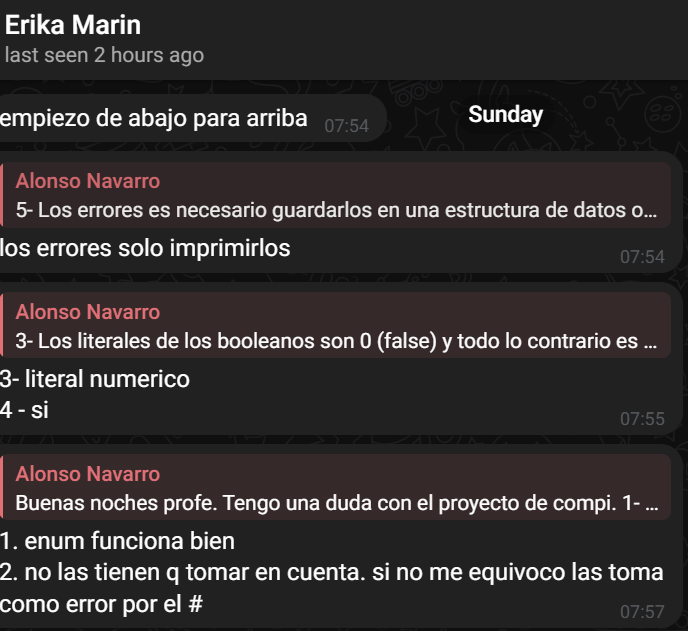
\includegraphics[width=0.5\textwidth]{respuestas-1.png}\par
\end{flushleft}

\subsection*{Fecha: 03-09-2024}
\begin{flushleft}
    La profesora responde la siguiente consulta:
    \begin{quote}
        Usted comentó que cosas como "1ejemplo", debería ser 
        un error y no que los separe como "1": literal y 
        "ejemplo": id. Hay otras cosas que se pegan, por 
        ejemplo con las directivas:
        
        \#include \textless stdio.h \textgreater
        
        lo separa como\par
        \#: error\par
        include: id\par
        \textless operador\par
        stdio: id\par
        . operador\par
        h: id\par
        \textgreater operador\par
        
        Entonces yo ya tengo definido el error genérico de 
        "1ejemplo", pero con esto estaba pensando en meter más 
        caracteres en ese mismo error, pero es que si fuera un 
        "5\textless identificador" en algún condicional ya croma.
    \end{quote}
    La respuesta de la profesora es:\par\vspace{1em}
    \centering
    
\includegraphics[width=0.5\textwidth]{respuestas-2.png}\par
\end{flushleft}

\subsection*{Fecha: 04-09-2024}
\begin{flushleft}
    \hspace*{2em} Luego de tener todo el scanner corriendo 
    correctamente se decide que lo siguiente es finalizar la 
    documentación. CV se encargará de la introducción, AN de 
    la estrategia de solución y VG de las lecciones aprendidas.
    Las demás secciones son redactadas en conjunto. Finalmente,
    se acuerda que cada integrante hará dos casos de prueba y 
    documentará lo encontrado.
\end{flushleft}

% Bibliografía
\newpage
\section*{Bibliografía}
\addcontentsline{toc}{section}{Bibliografía}
\begin{thebibliography}{9}

\bibitem{examplewebsite}
Klein, G., Rowe, S., \& Décamps, R. (marzo de 2023).
\emph{JFlex User’s Manual}.
JFlex Team.
En: \url{https://www.jflex.de/manual.html}.

\end{thebibliography}

\end{document}